% =====================================================================
% ภาคผนวก ก — ตัวอย่างส่วนติดต่อกับผู้ใช้ (คู่มือข้อ 19)
% แต่ละภาคผนวกเริ่มด้วย \chapter{ชื่อภาคผนวก} ใน main.tex
% ระบบใส่ "ภาคผนวก ก ข ค ..." ให้อัตโนมัติ และใช้ \section{...} ภายในได้ตามปกติ
% *** แทนภาพตัวอย่างด้วยภาพหน้าจอของระบบตนเอง ***
% =====================================================================
ภาคผนวกนี้แสดงหน้าจอหลักของระบบที่พัฒนาขึ้น

\section{หน้าเข้าสู่ระบบ}

หน้าเข้าสู่ระบบแสดงดังภาพที่~\ref{fig:ui-login}

\begin{figure}[H]
\centering
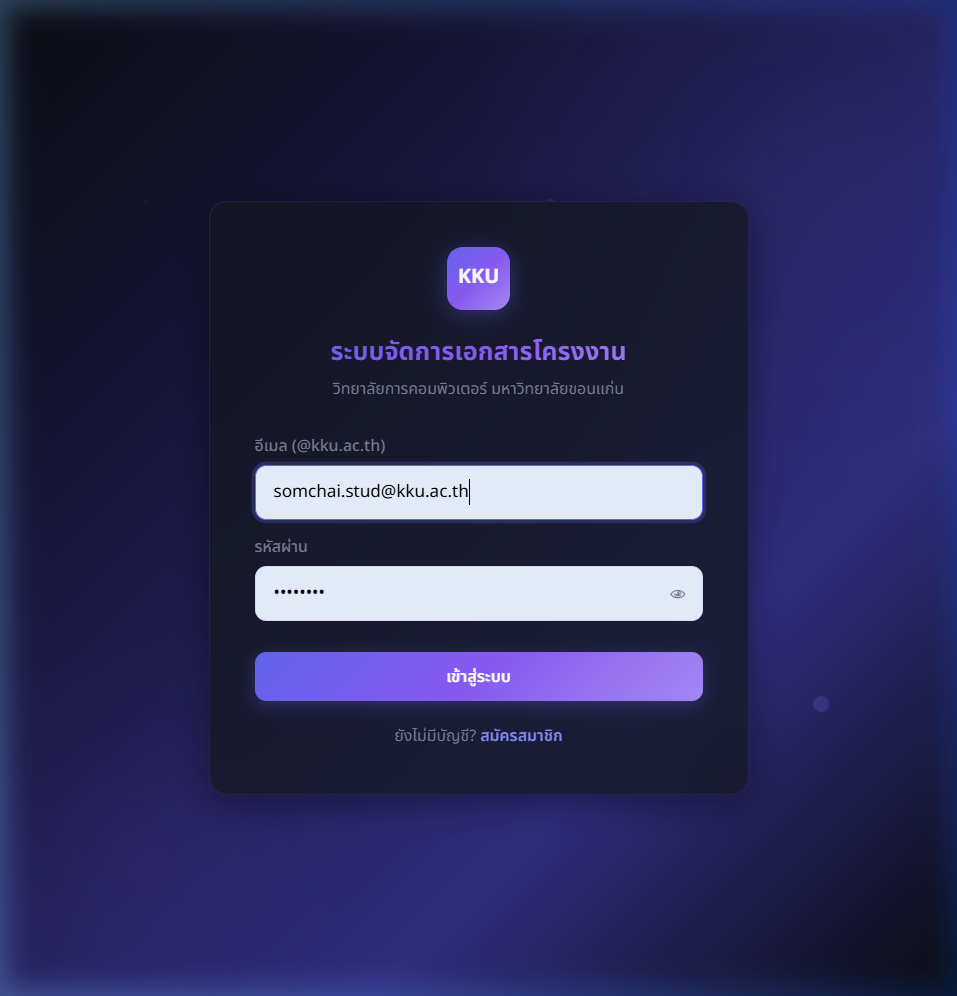
\includegraphics[width=0.5\linewidth]{images/ui-login.png}
\caption{หน้าเข้าสู่ระบบ}
\label{fig:ui-login}
\end{figure}

\section{หน้าหลัก}

หน้าหลักหลังเข้าสู่ระบบแสดงดังภาพที่~\ref{fig:ui-dashboard}

\begin{figure}[H]
\centering
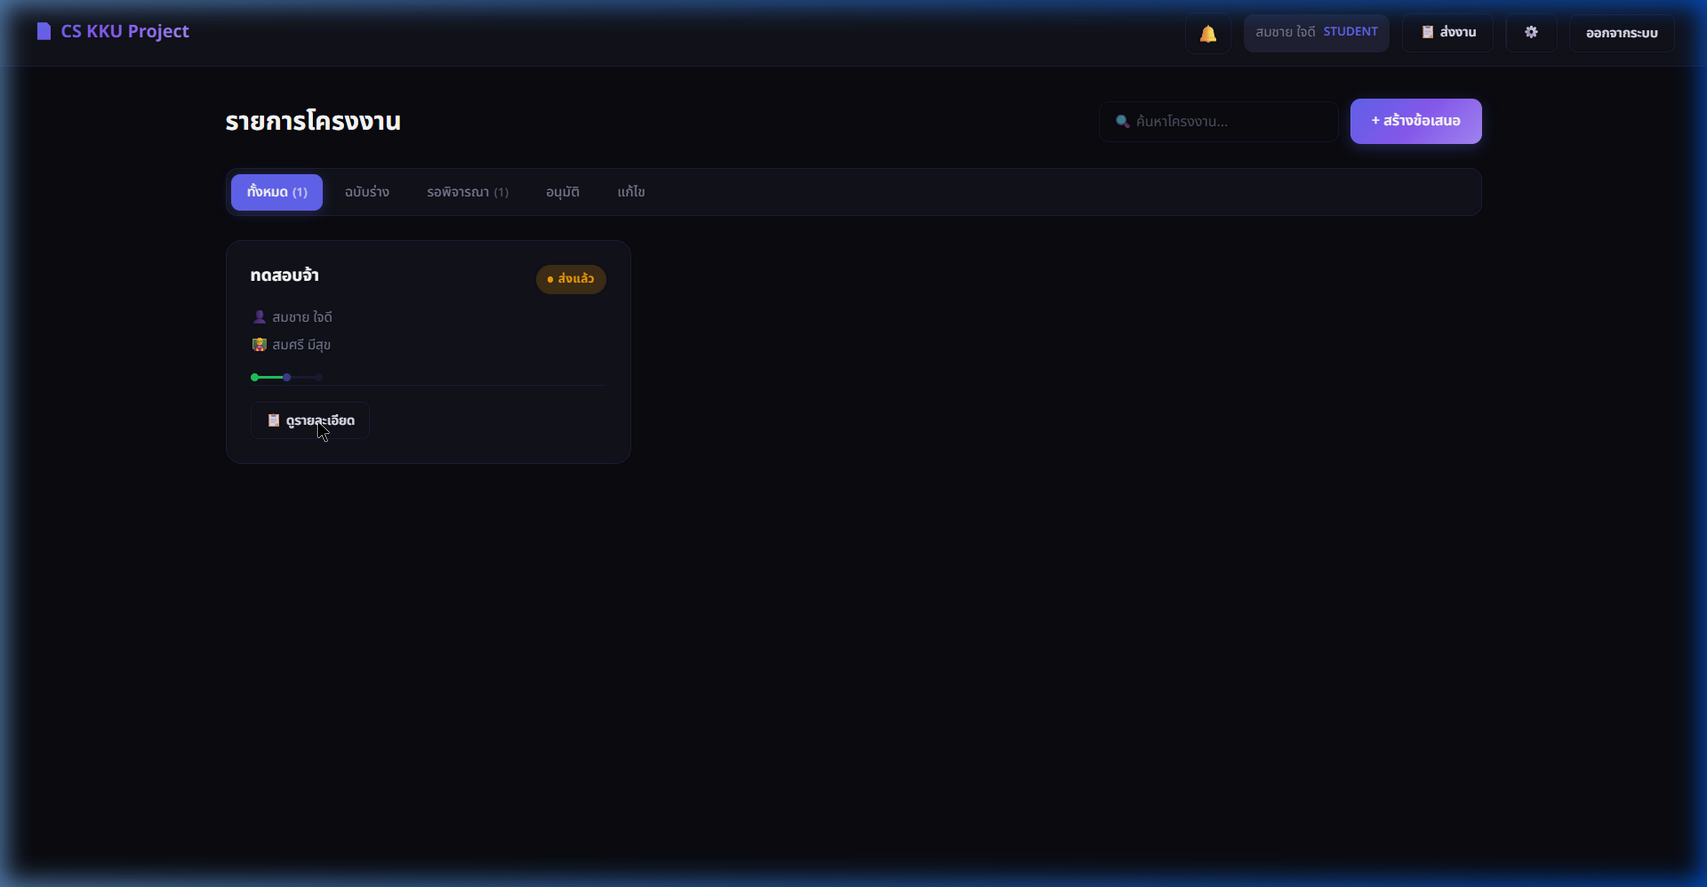
\includegraphics[width=0.95\linewidth]{images/ui-dashboard.png}
\caption{หน้าหลักของระบบ}
\label{fig:ui-dashboard}
\end{figure}
